% Configuration
\documentclass[a4paper, 10pt]{article}

% Formatting
\usepackage[landscape, left=0.75cm, top=1.0cm, right=0.75cm, bottom=1.5cm, footskip=15pt]{geometry}
\setlength{\columnsep}{0.5cm}
\usepackage{flowfram}
\ffvadjustfalse
\Ncolumn{3}
\usepackage[compact]{titlesec}
\usepackage{parskip}
\setlength{\parskip}{2pt}

% ------------------------
% Imports and commands
% ------------------------

% Language stuff
\usepackage[english]{babel}
\usepackage[utf8]{inputenc}

% Math stuff
\usepackage{amsthm}
\usepackage{amssymb}
\usepackage{amsmath}
\usepackage{bm}
\usepackage{centernot}
\usepackage{esint}

\newtheorem*{corollary}{Cor}
\newtheorem*{lemma}{Lemma}
\newtheorem*{proposition}{Prop}

\theoremstyle{definition}
\newtheorem*{theorem}{Thm}
\newtheorem*{definition}{Def}

% Colored boxes
\usepackage{xcolor}
\usepackage{mdframed}
\usepackage{framed}
\mdfsetup{skipabove=2pt,skipbelow=2pt}

% Fix for MDFramed
\makeatletter
\DeclareDocumentCommand{\mdtheorem}{ O{} m o m o }%
 {\ifcsdef{#2}%
   {\mdf@PackageWarning{Environment #2 already exits\MessageBreak}}%
   {%
    \IfNoValueTF {#3}%
     {%#3 not given -- number relationship
      \IfNoValueTF {#5}%
        {%#3+#5 not given
        \@definecounter{#2}%
        \expandafter\xdef\csname the#2\endcsname{\@thmcounter{#2}}%
        \newenvironment{#2}[1][]{%
          \refstepcounter{#2}%
          \ifstrempty{##1}%
            {\let\@temptitle\relax}%
            {%
             \def\@temptitle{\mdf@theoremseparator%
                             \mdf@theoremspace%
                             \mdf@theoremtitlefont%
                             ##1}%
             \mdf@thm@caption{#2}{{#4}{\csname the#2\endcsname}{##1}}%
             }%
          \begin{mdframed}[#1,frametitle={\strut#4\ \csname the#2\endcsname%
                                          \@temptitle}]}%
          {\end{mdframed}}%
        \newenvironment{#2*}[1][]{%
          \ifstrempty{##1}{\let\@temptitle\relax}{\def\@temptitle{\mdf@theoremseparator \mdf@theoremspace ##1}}% <- the problem was here
          \begin{mdframed}[#1,frametitle={\strut#4\@temptitle}]}%
          {\end{mdframed}}%
        }%
        {%#5 given -- reset counter
        \@definecounter{#2}\@newctr{#2}[#5]%
        \expandafter\xdef\csname the#2\endcsname{\@thmcounter{#2}}%
        \expandafter\xdef\csname the#2\endcsname{%
               \expandafter\noexpand\csname the#5\endcsname \@thmcountersep%
                  \@thmcounter{#2}}%
        \newenvironment{#2}[1][]{%
          \refstepcounter{#2}%
          \ifstrempty{##1}%
            {\let\@temptitle\relax}%
            {%
             \def\@temptitle{\mdf@theoremseparator%
                             \mdf@theoremspace%
                             \mdf@theoremtitlefont%
                             ##1}%
             \mdf@thm@caption{#2}{{#4}{\csname the#2\endcsname}{##1}}%
             }
          \begin{mdframed}[#1,frametitle={\strut#4\ \csname the#2\endcsname%
                                          \@temptitle}]}%
          {\end{mdframed}}%
        \newenvironment{#2*}[1][]{%
          \ifstrempty{##1}%
            {\let\@temptitle\relax}%
            {%
             \def\@temptitle{\mdf@theoremseparator%
                             \mdf@theoremspace%
                             \mdf@theoremtitlefont%
                             ##1}%
             \mdf@thm@caption{#2}{{#4}{\csname the#2\endcsname}{##1}}%
             }%
          \begin{mdframed}[#1,frametitle={\strut#4\@temptitle}]}%
          {\end{mdframed}}%
        }%
     }%
     {%#3 given -- number relationship
        \global\@namedef{the#2}{\@nameuse{the#3}}%
        \newenvironment{#2}[1][]{%
          \refstepcounter{#3}%
          \ifstrempty{##1}%
            {\let\@temptitle\relax}%
            {%
             \def\@temptitle{\mdf@theoremseparator%
                             \mdf@theoremspace%
                             \mdf@theoremtitlefont%
                             ##1}%
             \mdf@thm@caption{#2}{{#4}{\csname the#2\endcsname}{##1}}%
             }
          \begin{mdframed}[#1,frametitle={\strut#4\ \csname the#2\endcsname%
                                          \@temptitle}]}%
          {\end{mdframed}}%
        \newenvironment{#2*}[1][]{%
          \ifstrempty{##1}{\let\@temptitle\relax}{\def\@temptitle{:\ ##1}}%
          \begin{mdframed}[#1,frametitle={\strut#4\@temptitle}]}%
          {\end{mdframed}}%
     }%
   }%
 }
\makeatother

\definecolor{cwhite}{HTML}{d7dbd7}
\mdfdefinestyle{important}{
    linecolor=yellow,
    linewidth=0pt,
    innertopmargin=0pt,
    innerbottommargin=2pt,
    innerrightmargin=2pt,
    innerleftmargin=2pt,
    leftmargin=0pt,
    rightmargin=0pt,
    backgroundcolor=cwhite,
    frametitleaboveskip=1pt,
    frametitlebelowskip=1pt,
    theoremseparator={},
    theoremspace={},
}
\mdtheorem[style=important]{ntheorem}{}

\definecolor{bgold}{HTML}{FFED8A}
\mdfdefinestyle{trick}{
    linecolor=yellow,
    linewidth=0pt,
    innertopmargin=0pt,
    innerbottommargin=2pt,
    innerrightmargin=2pt,
    innerleftmargin=2pt,
    leftmargin=0pt,
    rightmargin=0pt,
    backgroundcolor=bgold,
    frametitleaboveskip=1pt,
    frametitlebelowskip=1pt,
    theoremseparator={},
    theoremspace={},
}
\mdtheorem[style=trick]{note}{}

% Table stuff
\usepackage{tabularx} % tabularx since the width should be handled automatically
\usepackage{booktabs}
\usepackage{makecell}

% Graph stuff
\usepackage{pgfplots}
\usepackage{tikz}
\usetikzlibrary{matrix}

% Miscellaneous
\usepackage{hyperref}
\hypersetup{colorlinks=true, urlcolor=blue, linkcolor=blue, citecolor=blue}

\usepackage{enumitem}
\setitemize{itemsep=0.5pt, topsep=0.5pt}
\setenumerate{itemsep=0.75pt, topsep=0.5pt}

\usepackage{graphics}

\newlist{exanswers}{itemize}{2}
\setlist[exanswers]{itemsep=2pt, topsep=2pt}
\setlist[exanswers,1]{label=$\diamond$,leftmargin=5mm}
\setlist[exanswers,2]{label=\textbullet,leftmargin=1mm}

% Custom commands
\newcommand{\R}{\mathbb{R}}
\newcommand{\Q}{\mathbb{Q}}
\newcommand{\N}{\mathbb{N}}
\newcommand{\Z}{\mathbb{Z}}
\newcommand{\C}{\mathbb{C}}
\newcommand{\J}{\mathcal{J}}
\newcommand{\BO}{\mathcal{O}}
\newcommand{\Hess}{\text{Hess}}
\renewcommand{\labelenumii}{\arabic{enumi}.\arabic{enumii}}
\newcommand{\defi}{\stackrel{\text{def}}{\iff}}

% Metadata
\title{Analysis II Summary}
\author{Nicola Studer \\ \href{mailto:nicstuder@student.ethz.ch}{nicstuder@student.ethz.ch}}
\date{\vspace{-5ex}}


% ------------------------
% Document
% ------------------------

\begin{document}
\maketitle

\section{Ordinary differential equations}
\[F(x, y^{(n)}, \ldots, y'(x), y(x)) = 0\]
Given a function \(F\) of \(x, y\), where \(y\) is a function itself. \(F\) is an implicit ODE of \textbf{order} \(n\).

\begin{note*}[Linear ODE's]
    \(y^{(k)} + a_{k-1}(x)y^{(k-1)} + \ldots + a_1(x)y' + a_0(x)y = b(x)\)
    with \(a_{k-1}, \ldots, a_0, b\) as cont. functions of \(x\) in \(I \subset \R\). If \(\bm{b = 0}\) then the ODE is called \textbf{homogeneous}.
\end{note*}

\begin{ntheorem*}[Properties of linear ODEs]
    \begin{enumerate}
        \item all coefficients are continuous functions
        \item no products of \(y\) and its derivatives
        \item no powers of \(y\) and its derivatives
        \item no functions which depend on \(y\) or its derivatives
        \item no leading coefficient in front of the highest derivative
    \end{enumerate}
\end{ntheorem*}

\begin{theorem}[Main result about linear ODEs]
    \(\;\)
    \begin{enumerate}
        \item Let \(\mathcal{S}_0\) be the set of solutions when \(b = 0\). Then \(\mathcal{S}_0\) is a vector space of dimension \(k\). If \(f_1, \ldots, f_k\) are the solutions, then so is \(a_1f_1+ \ldots a_kf_k\).
        \item For any \textbf{initial condition} (i.e. for any choice of \(x_0 \in I\)) there is a unique solution \(f \in \mathcal{S}_0\) such that: \\
        \(f(x_0) = y_0, f'(x_0) = y_1, \ldots, f^{(k-1)}(x_0) = y_{k-1}\)
        \item For any arbitrary \(b(x)\), the set of solutions of the ODE is \(\mathcal{S}_b = \{f + f_p \ | \ f \in \mathcal{S}_0\}\) where \(f_p\) is a particular solution of the ODE.
        \item For any initial condition there is a unique solution \(f \in \mathcal{S}_b\).
    \end{enumerate}
\end{theorem}

\begin{note*}[Solve initial value problem]
    \begin{enumerate}
        \item Solve ODE
        \item With initial values create LSE
    \end{enumerate}
\end{note*}

\pagebreak
\subsection{Linear ODE of order 1}
\begin{note*}[Solution and derivation]
        \(1.\) Solve the homogeneous ODE:
        \begin{align*}
            && y' + ay &= 0 & \\
            &\implies & y' &= - ay & \\
            &\implies & \tfrac{y'}{y} &= -a & (\text{assume \(y \neq 0\) no \(I\)}) \\
            &\implies & \ln(|y|) &= -A + C & (A(x) = \smallint a(x) \,dx) \\
            &\implies & y &= e^{-A + C} = z\cdot e^{-A} & (\text{simplify})
        \end{align*}
        \(2.\) Find \(f_p: I \to \C\) such that \(f'_p + a(x)f_p = b(x)\) with variation of parameters or undetermined coefficients.

        \(3.\) General solution: \(f(x) = f_h(x) + f_p(x)\)
\end{note*}

\subsubsection{Method of undetermined coefficients}
\begin{tabular}{|c|c|}
    \hline
    \(\bm{b(x)}\) & \textbf{Guess} \\
    \hline
    \(a e^{\alpha x}\) & \(c e^{\alpha x}\) \\
    \(P_n(x)\) & \(Q_n(x)\) \\
    \hline
    \makecell{\(a \sin(\beta x)\) \\ \(a \cos(\beta x)\)} & \(D \sin(\beta x) + E \cos(\beta x)\) \\
    \hline
    \makecell{\(a e^{\alpha x} \sin(\beta x)\) \\ \(a e^{\alpha x} \cos(\beta x)\)} & \(D e^{\alpha x} \sin(\beta x) + E e^{\alpha x} \cos(\beta x)\) \\
    \hline
    \(P_n(x) e^{\alpha x}\) & \(Q_n(x) e^{\alpha x}\) \\
    \hline
    \makecell{\(P_n(x) e^{\alpha x} \sin(\beta x)\) \\ \(P_n(x) e^{\alpha x} \cos(\beta x)\)} & \(e^{\alpha x} (Q_n(x) \sin(\beta x) + R_n(x) \cos(\beta x))\) \\
    \hline
\end{tabular}

\begin{enumerate}
    \item If \(b(x)\) is a linear combination of the basis functions, use corresponding linear combination of the functions.
    \item If \(f_p = f_0\), try to multiply it with \(x^m\) where \(m\) denotes the multiplicity of the eigenvalue.
\end{enumerate}

\subsubsection*{Variation of parameters}
\begin{enumerate}
    \item Assume \(f_p = z(x) \cdot e^{-A(x)}\) for a function \(z: I \to \C\)
    \item Insert the equation and construct \(z\):
    \begin{align*}
        &&y' + ay &= b \\
        &\implies& z'e^{-A} &= b \\
        &\implies& z' &= be^{A} \\
        &\implies& z &= \smallint b(x)e^{A(x)}\,dx \\
        &\implies& f_p &= \smallint b(t) e^{A(t)}\,dt \cdot e^{-A(x)}
    \end{align*}
\end{enumerate}

\subsubsection*{Integration Factor}
\begin{align}
    \tag{\(\dagger\)} \frac{dy}{dx} + a(x) y = b(x)
\end{align}
\begin{enumerate}
    \item Multiply both sides of (\(\dagger\)) with \(e^{A(x)} = e^{\smallint a(x)\,dx}\) \par
    \centering
    \(\frac{dy}{dx} e^{\smallint a(x)\,dx} + ya(x)e^{\smallint a(x)\,dx} = b(x)e^{\smallint a(x)\,dx}\)
    \item \raggedright Observe the product rule on the left hand side: \par
    \centering
    \(\frac{d}{dx}ye^{\smallint a(x)\,dx} = b(x)e^{\smallint a(x)\,dx}\)
    \item \raggedright Call \(y e^{\smallint a(x)\,dx}:=z(x) \implies y = z(x)e^{-A(x)}\) (\(\ddagger\)) \par
    \centering
    \(\frac{d}{dx}z(x) = b(x)e^{\smallint a(x)\,dx}\)
    \item \raggedright Solve for \(z(x)\): \(z(x) = \int b(x) e^{A(x)}\,dx\)
    \item \raggedright Insert (\(\ddagger\)):
    \(y = \left(\int b(x)e^{A(x)} \,dx\right) e^{-A(x)}\)
\end{enumerate}

\subsection{Linear ODE with constant coefficients}
\[Dy = b(x) \quad D = \frac{d^k}{dx^k} + a_{k - 1} \frac{d^{k-1}}{dx^{k-1}} + \ldots + a_0\]

\subsubsection*{1. Solve homogeneous equation}
Assume \(y = e^{\lambda x}\) for some \(\lambda \in \C\). We put that guess in the initial formula and get the following (simplified) form:
\[e^{\lambda x}(\lambda^k + a_{k-1}\lambda^{k-1} + a_{k-2}\lambda^{k-2} + \ldots + a_0) = e^{\lambda x} \cdot P(\lambda) = 0\]
Since \(e^{\lambda x}\) can never be \(0\) \(\implies\) \(P(\lambda) = 0\). \(P(\lambda)\) is the \textbf{characteristic polynomial} with its roots called \textbf{eigenvalues}.

\begin{theorem}
    \(D e^{\lambda x} = 0 \iff \lambda\) is a root of \(P_D(\lambda)\)
\end{theorem}

\begin{note*}[Solutions]
    The functions \(f_{i, l}: x \mapsto x^l e^{\lambda_i x}\) span the solution space \(S_0\) with \(0 \leq l < m\), \(m\) as the multiplicity of \(\lambda_i\).

    \begin{itemize}
        \item If \(\lambda = a + ib\) is EV of \(P(\lambda)\), then \(P(\overline{\lambda})\) is an EV.
        \item Complex root: \(e^{(a + bi) \cdot x} = e^{ax}[\cos(bx) + i \sin(bx)]\)
        \item If \(b = e^{\alpha x}\), but \(\alpha\) is a root of \(P(\lambda)\) with \(m = k\), then try \(zx^k \cdot e^{\alpha x}\) for \(y_p\)
    \end{itemize}
\end{note*}

\begin{ntheorem*}[Superposition Principle]
    \(D(y_1 + y_2) = D(y_1) + D(y_2) = b_1 + b_2\)
\end{ntheorem*}

\begin{ntheorem*}[Separation of variables]
    ODE separable if \(\frac{dy}{dx} = b(x)g(y) \implies \frac{dy}{g(y)} = b(x) \,dx\). If \(g(y) = 0\), then \(y = y_h\) otherwise integrate both sides.
\end{ntheorem*}

\section{Differential calculus in \(\R^n\)}
\subsection{Terminology}
\begin{tabular}{>{\bfseries}l l}
    Vector Field & \(f: \R^n \to \R^m \quad (m > 1)\) \\
    Scalar Field & \(f: \R^n \to \R\) \\
    Monomial & \(f :\begin{cases}
        \R^n \to \R \\
        (x_1, x_2, \ldots, x_n) \mapsto \alpha x_1^{d_1} x_2^{d_2} \ldots x_n^{d_n}
    \end{cases}\) \\
    Linear Map & \(f :\begin{cases}
        \R^n \to \R \\
        x \mapsto Ax \quad (A \in \C^{m \times n})
    \end{cases}\) \\
    Affine Map & \(f :\begin{cases}
        \R^n \to \R \\
        x \mapsto Ax + y_p \quad (y_p \in \R^m)
    \end{cases}\) \\
    Cart. Prod. & \(f :\begin{cases}
        \R^n \to \R^{s + t} \\
        x \mapsto (f_1(x), f_2(x))
    \end{cases}\) \\
\end{tabular}

\begin{ntheorem*}[Converges of sequences]
    \((x_k)_{k \in \N} \subset \R^n, \ y \in \R^n\). \(\lim\limits_{k \to \infty}x_k = y\)
    \begin{itemize}
        \item[\(\Leftrightarrow\)] \(\forall \epsilon > 0 \, \exists N \geq 1 \, \forall k \geq N: ||x_k - y|| < \epsilon\)
        \item[\(\Leftrightarrow\)] For each \(i\), \(1 \leq i \leq n\) the sequence \((x_{k, i}) \subset \R\) of real numbers converges to \(y_i \in \R\)
        \item[\(\Leftrightarrow\)] The sequence of real numbers \(||x_k - y|| \to 0\)
    \end{itemize}
\end{ntheorem*}

\begin{definition}
    \(f: X \subset \R^n \to \R^m\), \(x_0 \in X\).
    \(f\) \textbf{has a limit} \(y \in \R^m\) as \(x \to x_0\) (with \(x \neq x_0\)) if
    \begin{enumerate}
        \item \(\forall \epsilon > 0 \, \exists \delta > 0 \, \forall x \in X, x \neq x_0: ||f(x) - y|| < \epsilon\)
        \item \(\forall\) sequences \((x_k)\) in \(X\) with \(\lim x_k = x_0\) and \(x_k \neq x_0\) converges the sequence \(f(x_k)\) to \(y\).
    \end{enumerate}
\end{definition}

\begin{ntheorem*}[Continuity]
    \(f: X \to \R^m\) cont. at \(x_0\) if
    \begin{enumerate}
        \item \(\forall \epsilon > 0 \, \exists \delta > 0 \, \forall x \in X : \)
        \[||x-x_0|| < \delta \implies ||f(x) - f(x_0)|| < \epsilon\]
        \item \(\forall\)seq. \((x_k)\) with \(\lim x_k = x_0: \lim f(x_k) = f(x_0)\)
    \end{enumerate}
    \(f\) cont. on \(X\) if it is cont. \(\forall x_0 \in X\).
\end{ntheorem*}

\begin{corollary}
    \begin{enumerate}
        \item \(f_1: \R^n \to \R^m, f_2: \R^n \to \R^s\) cont., then \(f: (f_1, f_2): \R^n \to \R^{m + s}, x \mapsto (f_1(x), f_2(x))\) is cont.
        \item \(f: \R^n \to \R^m, x \mapsto (f_1(x), f_2(x), \ldots)\) cont.\\  \(\iff  \forall 1 \leq i \leq m \ f_i: \R^n \to \R\) are cont.
        \item \(f: \R^n \to \R^m, x \mapsto Ax\) and polynomials are cont.
        \item Sums/products of cont. functions are cont.
        \item Functions with separated variables are cont. if each variable is cont.
        \item Composition of cont. functions are cont.
        \item If \(f: \R^2 \to \R\) is cont. Fix \(y_0 \in \R\). \\ Define \(g_{y_0}(x) := f(x, y_0)\). Then \(g_{y_0}: \R \to \R\) is cont.
        \[\not\Rightarrow f: \R^2 \to \R \ \text{is cont.}\]
    \end{enumerate}
\end{corollary}

\begin{ntheorem*}[Sandwich lemma]
    \(f, g, h : \R^n \to \R\), \(\forall x \in \R^n: f(x) \leq g(x) \leq h(x)\)
    \[\lim_{x \to a} f(x) = L = \lim_{x \to a} h(x) \implies \lim_{x \to a}g(x) = L\]
\end{ntheorem*}

\begin{note*}[Polar Coordinates]
    For \(f: \R^2 \to \R\) polar coordinates are sometimes helpful.
    \(p = r \cos \theta \quad q = r \sin \theta\)
    \[\lim_{(x, y) \to (0, 0)}f(x, y) = \lim_{(r\cos\theta, r\sin\theta) \to (0,0)}f(p, q) = \ldots = \lim_{r \to 0} \zeta\]
\end{note*}

\subsection{Sets Bounds \(M \subseteq \R^n\)}
\vspace{-8pt}
\begin{align*}
    M \ \textbf{is bounded} \defi & \{||x|| \in \R \mid x \in M\} \ \text{is bounded} \\
    M \ \textbf{is open} \defi & \forall p \in M: \exists r \in \R^{>0}: B_p(r) \subseteq M \\
    \defi & \R^n \setminus M \ \text{is closed}\\
    M \ \textbf{is closed} \defi & \forall (x_k)_{k \in \N} \subseteq M \ \text{that converge to} \\
    & x \in \R^n: x \in M \\
    M \ \textbf{is compact} \defi& M \ \text{closed and bounded}
\end{align*}

\begin{note*}[Special Sets]
    \begin{itemize}
        \item \(\R^n\) and \(\emptyset\) are the \textbf{only} open and  closed sets of \(\R^n\).
        \item The open disc \(B_r(x_0) = \{x \in \R^n \mid |x - x_0| < r\}\) is bounded and open.
        \item The closed disc \(\overline{B_r(x_0)} = \{x \in \R^n \mid |x - x_0| \leq r\}\) is closed.
        \item \(I_1 \times \ldots I_n\) is closed (compact) if each interval \(I_i\) is closed (compact)
    \end{itemize}
\end{note*}

\begin{theorem}
    \(f: \R^n \to \R^m\) cont. \(\forall Y \subseteq \R^m\) \textbf{closed}, the set \(f^{-1}(Y) = \{x \in \R^n \mid f(x) \in Y\}\) is closed.
\end{theorem}

\begin{theorem}
    \(f: \R^n \to \R^m\) cont. \(\forall Y \subseteq \R^m\) \textbf{open}, the set \(f^{-1}(Y) = \{x \in \R^n \mid f(x) \in Y\}\) is open.
\end{theorem}

\begin{ntheorem*}[Min-Max theorem]
    \(X \subseteq \R^n\) compact. \(f: X \to \R\) cont. \(\implies\)
    \[\exists x_+, x_- \in X: f(x_+) = \sup_{x \in X}(f(x)), \quad f(x_-) = \inf_{x \in X} f(x)\]
\end{ntheorem*}

\subsection{Partial derivatives}
\begin{definition}
    \(f: X \subseteq \R^n \to \R\), \(X\) open. The \textbf{partial derivative} of \(f\) with respect to \(x_i\) at the point \(a \in \R^n\) is
    \[\frac{\partial f}{\partial x_i}(a) = \lim_{h \to 0} \frac{f(a + h e_i) - f(a)}{h} \hfill \ \ ((e_i)_j = \delta_{ji}, j = 1, \ldots, n)\]

    If \(f: X \to \R^m\) for \(x_0 \in \R^n\), then
    \[\frac{\partial f}{\partial x_i}(a) = \begin{bmatrix}
        \frac{\partial f_1}{\partial x_i}(a) \\
        \vdots \\
        \frac{\partial f_m}{\partial x_i}(a)
    \end{bmatrix}\]
\end{definition}

\begin{corollary}
    \(X \subseteq \R^n\) open, \(f, g: X \to \R^m\):
    \begin{itemize}
        \item \(\partial_{x_i}(f + g) = \partial_{x_i}(f) + \partial_{x_i}(g)\)
        \item \(\partial_{x_i}(f \cdot g) = \partial_{x_i}(f) \cdot g + f \cdot \partial_{x_i}(g)\) if \(m = 1\)
        \item \(\partial_{x_i}(f / g) = (\partial_{x_i}(f) \cdot g - f \cdot \partial_{x_i}(g)) / g^2\) if \(m = 1, g \not\equiv 0\)
    \end{itemize}
\end{corollary}

\begin{definition}
    The \textbf{Jacobi Matrix} of \(f: X \subset \R^n \to \R^M\) at \(x \in X\):
    \[\J_f(x) = \begin{bmatrix}
        \frac{\partial f_i}{\partial x_j}(x)
    \end{bmatrix}_{\substack{1 \leq i \leq m \\ 1 \leq j \leq n}}\]
\end{definition}

\begin{definition}
    \(f: X \subseteq \R^n \to \R\), \(X\) open. The \textbf{gradient} of \(f\):
    \[\nabla f(x) = \J_f(x)^\top\]
    The gradient points in the direction of greatest increase and is perpendicular to the level set.
\end{definition}

\subsection{The differential}
\begin{definition}
    \(f: \R^n \to \R^m\) is diff. at \(x_0\), with \textbf{differential} \(u\), if there exists a linear map \(u: \R^n \to \R^m\) such that
    \[\lim_{\substack{x \to x_0 \\ x \neq x_0}} \frac{f(x) - (f(x_0) + u(x - x_0))}{||x-x_0||} = 0\]

    The linear map \(u: \R^n \to \R^m\) is called (total) \textbf{differential} of \(f\) at \(x_0\), denoted by \(df(x_0), d_{x_0}f\)
\end{definition}

\begin{theorem}
    \(f, g: \R^n \to \R^m\) diff. at \(x_0 \implies\)
    \begin{enumerate}
        \item \(f\) is cont. at \(x_0\)
        \item \(f\) admits partial derivatives on \(x_0\) w.r.t each variable
        \item \(\J_f(x_0)\) is the differential w.r.t the standard basis.
        \item \(d_{x_0}(f \pm g) = d_{x_0}f \pm d_{x_0}g\)
        \item \(d_{x_0}(f \cdot g) = (d_{x_0}f)g(x_0) + f(x_0) \cdot (d_{x_0} g)\) if \(m = 1\)
        \item If \(m = 1\) and \(g \not\equiv 0\), the \(f / g\) is diff.
    \end{enumerate}
\end{theorem}

\begin{ntheorem*}[Multivaraible Chain Rule]
    Let \(X \subseteq \R^n\) and \(Y \subseteq \R^m\) be open \(f: X \to Y, g: T \to \R^p\) diff functions, then
    \[d_{x_0}(g \circ f) = d(g \circ f)(x_0) = dg(f(x_0)) \circ df(x_0)\]
    The Jacobian satisfies: \(\J_{g \circ f}(x_0) = \J_g(f(x_0)) \cdot \J_f(x_0)\)
\end{ntheorem*}

\begin{ntheorem*}[Partial Convergence]
    If \(f : X \to \R^m\) has all partial derivatives \(\frac{\partial f_i}{\partial x_j}: X \to \R^m\) and if these functions are cont. in \(X\) \(\implies\) \(f\) is diff. on \(X\).
\end{ntheorem*}

\begin{definition}
    The \textbf{tangent space} at \(x_0\) is the graph of the affine linear map
    \[g(x) = f(x_0) + (d_{x_0}f)(x - x_0) \ \text{i.e} \ \{(x, g(x)) \in \R^n \times \R^m\}\]
\end{definition}

\begin{definition}
    \(X \subseteq \R^n\) open, \(f: X \to \R^m\), \(v \in \R^n \neq 0\), \(x_0 \in X\). The \textbf{directional derivative} in direction \(v\) is

    \resizebox{\linewidth}{!}{
        \(\lim_{t \to 0} \frac{f(x_0 + tv) - f(x_0)}{t} = \frac{d}{dt} f(x_0 + tv) \bigg|_{t=0} = d_vf(x_0) = \J_f(x_0) \cdot v\)
    }
\end{definition}

\begin{note*}[Summed up]
    \begin{itemize}
        \item \(f\) differentiable \(\implies f\) continuous
        \item \(f\) has all partial derivatives \(\centernot\implies f\) continuous
    \end{itemize}
\end{note*}

\subsection{Higher order partial derivatives}
\begin{definition}
    \(X \subset \R^n\) open, \(f: X \to \R^m\). We say \(f\) is diff. of class \(C^1\) if \(f\) is diff. on \(X\) and all its partial derivatives are continuous.

    The set of all \(C^1\) functions are denoted by \(C^1(X ; \R^m)\).

    Let \(k \geq 2\), then \(f \in C^k(X; R^m)\) if its diff. and each \(\partial_{x_i}f \in C^{k - 1}(X; \R^m)\).

    \(f\) is smooth or \(C^\infty\) if \(f \in C^k(X; \R^m) \ \forall k\).
\end{definition}

\begin{note*}[Known \(C^\infty\) functions]
    All polynomials, trigonometric and exponential functions
\end{note*}

\begin{ntheorem*}[Mixed derivatives commute]
    If \(f \in C^k\), \(k \geq 2\) then the partial derivatives of oder \(\leq k\) are independent of the order of differentiation.
    \[\frac{\partial}{\partial x_{i_k}} \dots \left(\frac{\partial}{\partial x_{i_2}}\left(\frac{\partial f}{\partial x_{i_1}}\right)\right) = \frac{\partial^k f}{\partial x_{i_k} \cdot \ldots \cdot \partial x_{i_2} \cdot \partial x_{x_{i_1}}}\]
\end{ntheorem*}

\begin{definition}[Hessian]
    \(f: X \to \R, X \subset \R^n\). If \(f \in C^2(X;\R)\), \(x_0 \in X\) the Hessian matrix of \(f\) at \(x\) is the symmetric square matrix
    \[\Hess_f(x_0) = \nabla^2 f(x_0) = \begin{bmatrix}
        \frac{\partial^2 f(x_0)}{\partial x_i \partial x_j}
    \end{bmatrix}_{\substack{1 \leq i \leq n \\ 1 \leq j \leq n}}\]
\end{definition}

\begin{ntheorem*}[Taylor Polynomial for \(f: \R^n \to \R\)]
    Approximation of \(f(y)\) for \(y\) close to \(x_0\).
    \begin{align*}
        T_1 f(x_0; y) &= f(x_0) + \nabla f(x_0) \cdot y \\
        &= f(x_0) + \frac{\partial f}{\partial x_1} (x_0) y_1 + \ldots \frac{\partial f}{\partial x_n} (x_0) y_n
    \end{align*}
    \begin{align*}
        T_2 f(x_0; y) = & f(x_0) + \nabla f(x_0) \cdot y \\
        & \frac{1}{2!} y \cdot \Hess_f(x_0) \cdot y^\top
    \end{align*}
    \begin{multline*}
        T_kf(x_0;y) = f(x_0) + \sum_{i = 1}^n \frac{\partial f}{\partial x_i} (x_0) y_i + \ldots + \\ \sum_{m_1 + \ldots m_n = k} \frac{1}{m_1! \cdot m_2! \cdot m_n!} \frac{\partial^k f}{\partial x_1^{m_1} \ldots \partial x_n^{m_n}}(x_0) \cdot y_1^{m_1 \ldots y_n^{m_n}}
    \end{multline*}
\end{ntheorem*}

\begin{note*}[Taylor Polynomials w/ Einstein Sum Convention]
    % \resizebox{\linewidth}{!}{
    \(T_kf(x_0;y) = f(x_0) + (\partial_if)(x_0)y_i + \frac{1}{2!}(\partial_{ij}f)(x_0)y_iy_j \newline + \frac{1}{3!}(\partial_{ijk}f)y_iy_jy_k + \cdots\)
    % }
\end{note*}

\begin{ntheorem*}[Taylor Approximation]
    Let \(f \in C^k(X; \R), x_0 \in X\)
    \[f(x) = T_k f(x_0, x - x_0) + E_k(f, x, x_0)\]
    which implies
    \[\lim_{x \to x_0} \frac{E_k(f, x, x_0)}{||x - x_0||^2} = 0\]
\end{ntheorem*}

\pagebreak
\subsection{Critical points}
\begin{definition}
    \(x_0 \in X\) of \(f: X \subseteq \R^n \to \R\) is a \textbf{local} maximum if there is a neighborhood \(B_{x_0}(r) := \{x \in \R^n \mid ||x - x_0|| < r\} \subseteq X \) such that \(\forall x \in B_{x_0}(r): f(x) \leq f(x_0)\). Vice versa for minimum.
\end{definition}

\begin{definition}
    \(x \in X\) is called a \textbf{critical point} of \(f\) if \(\nabla f(x_0) = 0\). These are candidates for local extrema. A critical point which is not an extrema is called  \textbf{saddle point}.
\end{definition}

\begin{theorem}
    \(f: X \subset R^n \to \R\) diff. on the interior of \(X\) and \(X\) closed and bounded, then a \textbf{global} extrema of \(f\) exists and is either at a point \(x_0 \in\) interior of \(X\) for which \(\nabla f(x_0) = 0\) or \(x_0 \in\) boundary of \(x\).
\end{theorem}

\begin{definition}[Non-degenerate critical point of \(f \in C^2(X, \R)\)]
    \[\det(\Hess_f(x_0)) \neq 0\]
\end{definition}

\begin{note*}[Special case for non-degenerate points]
    If \(\nabla f(x_0) = 0\), but also \(\det \Hess_f(x_0) = 0\), then we have to calculate each case individually.
\end{note*}

\begin{theorem}
    \(f: X \subset \R^n \to \R\), \(f \in C^2(X, \R)\). Let \(x_0 \in X\) be a critical point of \(f, \nabla f(x_0) = 0\). Then
    \begin{enumerate}
        \item \(\Hess_f(x_0)\) pos. def. \(\implies\) loc. min.
        \item \(\Hess_f(x_0)\) neg. def. \(\implies\) loc. max.
        \item \(\Hess_f(x_0)\) indefinite \(\implies\) saddle point.
    \end{enumerate}
\end{theorem}

\begin{note*}[Definiteness of matrices]
    A matrix \(A\) is \textbf{positive definite}
    
    \(\iff xAx^\top > 0 \quad \forall x \in \R^n\)

    \(\iff\) all eigenvalues of \(A\) are positive

    \(\iff\) all principal minors of \(A\) are positive:

    \begin{tabular}{c m{4cm}}
        \begin{tikzpicture}[baseline,>=latex]
            \matrix[
                matrix of math nodes,
                nodes in empty cells,
                left delimiter={[},
                right delimiter={]},
                nodes={text height=8pt,text depth=2pt,text width=10pt}
            ] (mat)
            {
            a & b & c  \\
            b & d & e  \\
            c & e & f  \\
            };
            \foreach \Valor in {1,...,3}
            \draw (mat-\Valor-1.south west) -| (mat-1-\Valor.north east);
        \end{tikzpicture}
        & \begin{enumerate}
            \vspace{15pt}
            \item \(a > 0\)
            \item \(ae - b^2 > 0\)
            \item \(\det(A) > 0\)
        \end{enumerate} \\
    \end{tabular}

    \(A\) is \textbf{negative definite} \(\iff -A\) positive definite

    \(A\) is \textbf{indefinite} \(\iff\) \(A\) neither pos. nor neg. def.
\end{note*}


\begin{corollary}[Closed form expression for \(3 \times 3\) matrix] \ \\
    \resizebox{\linewidth}{!}{
        \(\det \begin{bmatrix}
            a & b & c  \\
            d & e & f  \\
            g & h & i  \\
        \end{bmatrix} = a \cdot \det \begin{bmatrix}
            e & f \\
            h & i \\
        \end{bmatrix} - b \cdot \det \begin{bmatrix}
            d & f \\
            g & i \\
        \end{bmatrix} + c \cdot \det \begin{bmatrix}
            d & e \\
            g & h
        \end{bmatrix}\)
    }
\end{corollary}

\subsection{Change of variables}
\begin{definition}[Change of variables]
    \(X \subset \R^n\) open, \(f: X \to \R^n\) diff. \(f\) is a change of variables around \(x_0\) if there is a radius \(r > 0\), such that the restriction of \(f\) to the ball \(B_r(x_0) := \{x \in \R^n \ | \ ||x - x_0|| < r\}\) has the property that the image \(Y = f(B_r(x_0))\) is open in \(\R^n\) and there exists a differentiable map \(g: Y \to B\) s.t. \(f \circ g = id = g \circ f\).
\end{definition}

\begin{ntheorem*}[Inveres function theorem]
    \(X \subseteq \R^n\) open, \(f: X \to \R^n\) diff. If \(x_0 \in X\) is such that \(\det(\J_f(x_0)) \neq 0\), then \(f\) is a change of variables around \(x_0\). Moreover the Jacobian of \(g\) is determined by
    \[\J_g(f(x_0)) = \J_f(x_0)^{-1}\]
    Analogous of the fact that if \(f' > 0\) (or \(f' < 0\)) for a function \(f: I \subseteq \R \to \R\), then \(f\) is bijective.
\end{ntheorem*}

\subsubsection{Important change of variables (coordinates)}
\begin{enumerate}[leftmargin=0pt]
    \item \textbf{Polar}  \(f :\begin{cases}
        [0, \infty) \times [0, 2\pi) \to \R^2 \\
        (r, \theta) \mapsto (r \cos \theta, r \sin \theta)^\top
    \end{cases}\)
    
    The Jacobian of the change of variable is given by:
    \[\J_f(r, \theta) = \begin{bmatrix}
        \cos \theta & -r \sin \theta \\
        \sin \theta & r \cos \theta
    \end{bmatrix} \quad \det \J_f(r, \theta) = r\]

    \item \textbf{Cylindrical}  \(f :\begin{cases}
        [0, \infty) \times [0, 2\pi) \times \R \to \R^3 \\
        (r, \theta, z) \mapsto (r \cos \theta, r \sin \theta, z)^\top
    \end{cases}\)
    
    The Jacobian of the change of variable is given by:
    \[\J_f(r, \theta, z) = \begin{bmatrix}
        \cos \theta & -r \sin \theta & 0\\
        \sin \theta & r \cos \theta & 0 \\
        0 & 0 & 1 \\
    \end{bmatrix} \quad \det \J_f(r, \theta) = r\]

    \item \textbf{Spherical} \(f :\begin{cases}
        [0, \infty) \times [0, 2\pi) \times [0, \pi] \to \R^3 \\
        (r, \theta, \varphi) \mapsto (r \cos \theta \sin \phi, r \sin \theta \sin \phi, r \cos \phi)
    \end{cases}\)
    
    The Jacobian of the change of variable is given by:
    \begin{gather*}
        \J_f(r, \theta, z) = \begin{bmatrix}
            \cos \theta \sin \varphi & -r \sin \theta \sin \varphi & r \cos \theta \cos \varphi \\
            \sin \theta \sin \varphi & r \cos \theta \sin \varphi & r \sin \theta \cos \varphi \\
            \cos \varphi & 0 & -r \sin \varphi
        \end{bmatrix} \\
        \det \J_f(r, \theta) = r^2 \sin \varphi
    \end{gather*}
\end{enumerate}

\section{Integration in \(\R^n\)}
\begin{definition}
    \(\int_a^b f(x) \, dx = \begin{bmatrix}
        \int_a^b f_1(x) \, dx \\
        \vdots \\
        \int_a^b f_n(x) \, dx \\
    \end{bmatrix}\) for \(f: \R \to \R^n\)
\end{definition}

\subsection{Line Integrals}
\begin{definition}
    A \textbf{parameterized curve} \(\gamma: [a, b] \to \R^n\) is a continuous map and piecewise in \(C^1\) i.e. \(\exists k > 1\) and a partition \(a = t_0 < t_1 < \ldots < t_k = b\) s.t. \(\gamma \big|_{]t_{j-1}, t_j[}\) is \(C^1\) for \(1 \leq j \leq k\). \(\gamma(t)\) is a parameterization of the curve \(\text{Im} \gamma = \gamma([a, b])\).
\end{definition}

\begin{definition}
    Let \(\gamma: [a, b] \to \R^n\) be a parameterized curve in \(\R^n\). \(X \subset \R^n\) a subset of \(\R^n\) which contains the image of \(\gamma\). \(f: X \to \R^n\) a continuous function. The integral
    \[\int_a^b \langle f(\gamma(t)), \gamma'(t)\rangle \, dt \quad \text{denoted} \ \int_\gamma f(s) \cdot \, ds\]
    is called the line or path integral of \(f\) along \(\gamma\).
\end{definition}

\begin{definition}
    Let \(\gamma: [a, b] \to \R^n\) be a parameterized curve. An \textbf{oriented reparameterization} of \(\gamma\) is a parameterized curve \(\sigma: [c, d] \to \R^n\) such that \(\sigma = \gamma \circ \varphi\), where \(\varphi: [c, d] \to [a, b]\) is a cont. map, diff. on \(]a, b[\) that is strictly increasing and satisfies \(\varphi(a) = c\) and \(\varphi(b) = d\). Also \(\gamma = \sigma \circ \varphi^{-1}\)
\end{definition}

\begin{ntheorem*}[Properties of the line intergral]
    \begin{enumerate}[leftmargin=15pt]
        \item Only dependent on the image of the curve \(\gamma\). If \(\sigma\) is an oriented reparameterization of \(\gamma\), then
        \[\int_\gamma f(s) \cdot ds = \int_\sigma f(s) \cdot ds\]
        \item Let \(\gamma_1 + \gamma_2\) be the concatenation of these two curves. \((\gamma_1 + \gamma_2)(t) := \begin{cases}
            \gamma_1(t) & t \in [a, b] \\
            \gamma_2(t - b + c) & t \in [b, d + b - c]
        \end{cases}\)
        \[\int_{\gamma_1 + \gamma_2} f(s) \cdot ds = \int_{\gamma_1} f(s) \cdot ds + \int_{\gamma_2} f(s) \cdot ds\]
        \item Let \(-\gamma: t \mapsto \gamma(a + b - t)\) be the line in opposite direction
        \[\int_{-\gamma} f(s) \cdot ds = - \int_\gamma f(s) \cdot ds\]
    \end{enumerate}
\end{ntheorem*}

\begin{definition}
    A differentiable function \(g: X \subset \R^n \to \R\), such that \(\nabla g = f, f : X \to \R^n\) is called a \textbf{potential} for \(f\).
\end{definition}

\begin{note*}[Usefulness of potentials]
    Let \(g\) be a potential of \(f\), then
    \[\int_\gamma f(s) \cdot ds = \int_\gamma \nabla g(s) \cdot ds = g(\gamma(b)) - g(\gamma(a)).\]
    Thus the path integral of \(f\) only depends on the values of \(g\) at the end points of the curve.
\end{note*}

\begin{definition}
    Let \(X \subseteq \R^n\) and \(f: X \to \R^n\) a continuous vector field. If for any \(x_1, x_2 \in X\) the line integral \(\int_\gamma f(s) \cdot ds\) is independent of the choice of the curve \(\gamma\), then \(f\) is called \textbf{conservative}.
\end{definition}

\begin{ntheorem*}[Important equivalences]
    \(f: X \to \R^n\) is conservative
    \begin{enumerate}
        \item[\(\stackrel{\text{def}}{\iff}\)] The line integral of \(f\) is independent of the path
        \item[\(\iff\)] \(f = \nabla g\) for a \(g: X \to \R\) (i.e. \(f\) has a potential)
        \item[\(\iff\)] \(\int_\gamma f(s) \cdot ds = 0\) for any closed \(\gamma\)
    \end{enumerate}
\end{ntheorem*}

\begin{theorem}
    \(f: X \subseteq \R^n \to \R^n, C^1\) vector field and \(X\) open.
    \[f \ \text{conservative} \implies \frac{\partial f_j}{\partial x_i} = \frac{\partial f_i}{\partial x_j} \ \text{for} \ 1 \leq i, j \leq n\]
\end{theorem}

\begin{definition}
    \(f: X \subseteq \R^3 \to \R^3, C^1\), then the curl of \(f\) is defined as
    \[\text{curl}(f) := \begin{pmatrix}
        \partial_y f_3 - \partial_z f_2 \\
        \partial_z f_1 - \partial_x f_3 \\
        \partial_x f_2 - \partial_y f_1
    \end{pmatrix}\]
\end{definition}

\begin{theorem}
    \(f: \R^3 \to \R^3\) \(f\) conservative \(\implies \text{curl}(f) = 0\)
\end{theorem}

\begin{definition}
    A subset \(X \subseteq \R^n\) is \textbf{star shaped} if \(\exists x_0 \in X\) such that \(\forall x \in X\) the line segment of \(x\) to \(x_0\) is contained in \(X\).
\end{definition}

\begin{definition}
    A subset \(X \subseteq \R^n\) is convex, when for any \(x, y \in X\) the line segment from \(x\) to \(y\) is contained in \(X\).
    \[\text{convex} \implies \text{star-shaped}\]
\end{definition}

\begin{theorem}
    If \(X\) star-shaped open and \(f \in C^1\) vector field. Then
    \begin{gather*}
        \frac{\partial f_i}{\partial x_j} = \frac{\partial f_j}{\partial x_i} \ \forall 1 \leq i, j \leq n \implies f \ \text{is conservative} \\
        \text{curl}(f) = 0 \implies f \ \text{is conservative}
    \end{gather*}
\end{theorem}

\subsection{Riemann Integrals}
\begin{definition}
    A \textbf{rectangle} in \(\R^n\) is a product
    \[Q := [a_1, b_1] \times \ldots \times [a_n, b_n] = \prod_{j=1}^n I_i\]
    of \(n\) intervals \(I_i = [a_i, b_i]\) (not necessarily closed), and
    \[\text{vol}(Q) := \int_Q 1 \,dx = \prod_{i=1}^n (b_i - a_i).\]
\end{definition}

\begin{definition}
    Let \(P\) be a partition (collection) of \(Q = Q_1, \ldots, Q_k\) s.t. \(Q = \bigcup_{i=1}^k Q_i\) and all \(Q_i\) are pairwise disjoint and consider \(f: \R^n \to \R\).
    The upper/lower Riemann sum are defined as:
    \[L(P, f) = \sum_{j = 1}^k (\inf_{Q_j} f) \cdot \text{vol}(Q_j), \ U(P, f) = \sum_{j = 1}^k (\sup_{Q_j} f) \cdot \text{vol}(Q_j)\]
    and we define the lower and upper Riemann integral as
    \[\underline{\text{I}}(f) := \sup_P \{L(P, f)\}, \ \overline{\text{I}}(f) = \inf_P \{U(P, f)\}\]
\end{definition}

\begin{definition}
    \(f: Q \to \R\) is called \textbf{integrable} if \(\underline{\text{I}}(f) = \overline{\text{I}}(f)\).
    \[\int_Q f \,dx = \int_Q f(x_1, \ldots, x_n) \, dx_1 \ldots dx_n\]
\end{definition}

\begin{theorem}
    \(f\) is cont. and bounded on \(Q\), then \(f\) is integrable.
\end{theorem}

\begin{ntheorem*}[Properties] \(f,g : Q \subseteq \R^n \to \R\) integrable and \(\alpha, \beta \in \R\)
    \begin{enumerate}[leftmargin=15pt]
        \item \textbf{Linearity}: \(\int_Q(\alpha f + \beta g) \, dx = \alpha \int_Q f \, dx + \beta \int_Q g \,dx\)
        \item \textbf{Positivity}: If \(f \leq g\), then \(\int_Q f \, dx \leq \int_Q g \, dx\)
        \item \textbf{Upper bound}: \(| \int_Q f \, dx | \leq \int_Q |f| \, dx\)
        \item \textbf{Zero}: If \(f \geq 0\), then \(\int_Q f \, dx \geq 0\)
        \item \textbf{Triangle Ine.:} \(| \int_Q (f + g) \, dx | \leq \int_Q |f| \, dx + \int_Q |g| \, dx\)
        \item \textbf{Domain additivity}: If \(X_1\) and \(X_2\) are compact subsets of \(\R^n\) and \(f\) is continuous on \(X_1 \cup X_2\), then
        \[\int_{X_1 \cup X_2} f \, dx = \int_{X_1} f \, dx + \int_{X_2} f \, dx - \int_{X_1 \cap X_2} f \, dx\]
    \end{enumerate}
\end{ntheorem*}

\begin{ntheorem*}[Fubini's theorem]
    If \(Q = [a_1, b_1] \times \ldots \times [a_n, b_n]\), \(f: Q \to \R\) cont, then
    \[\int_Q f(x) \, dx = \int_{a_1}^{b_1} \left(\int_{a_2}^{b_2} \ldots \left( \int_{a_n}^{b_n} f(x) \, dx_n \right) \ldots dx_2\right) dx_1\]
    The order of integration is irrelevant.
\end{ntheorem*}

\begin{ntheorem*}[Fubini's theorem for general regions]
    \(X \subseteq \R_n\), \(f: X \to \R\), \(n_1, n_2 \geq 1\) and \(n = n_1 + n_2\), then for \(x \in \R^n = (x_1 \in \R^{n_1}, x_2 \in \R^{n_2})\), define
    \begin{align*}
        X_{x_1} &:= \{x_2 \in \R^{n_2} \mid (x_1, x_2) \in X\} \subseteq \R^{n_2} \\
        X_1 &:= \{x_1 \in \R^{n_1} \mid X_{x_1} \neq \emptyset\} \subseteq \R^{n_1}
    \end{align*}
    If \(g(x_1):= \int_{X_{x_1}} f(x_1, x_2) \, dx_2\) is continuous on \(X_1\), then
    \[\int_X f(x) \, dx = \int_{X_1} g(x_1) \, dx_1 = \int_{X_1}\int_{X_{x_1}} f(x_1, x_2) \, dx_2 \, dx_1\]
\end{ntheorem*}

\begin{definition}
    For \(1 \leq m \leq n\) a \(m\)-parameterized set or parameterized \(m\)-set is a continuous function \(\varphi: [a_1, b_1] \times \ldots \times [a_m, b_m] \to \R^n\) which is \(C^1\) on \((a_1, b_1) \times \ldots \times (a_m, b_m)\).
    If \(m = 1\) then \(\varphi\) is a parameterized curve in \(\R^n\).
\end{definition}

\begin{definition}
    A set \(Y \subseteq \R^n\) is called negligible if \(\exists\)finitely many \(\varphi_i\), parameterized \(m_i\)-sets with \(m_i \leq n\) such that \(1 \leq i \leq k\)
    \[Y \subseteq \bigcup_{i = 1}^k \varphi_i(x_i)\]
    where \(\varphi_i: x_i \to \R^n\)
\end{definition}

\begin{theorem}
    If \(Y \subseteq \R^n\) is negligible closed bounded then
    \[\int_Y f(x_1, \ldots, x_n) \, dx_1 \, \ldots dx_n = 0\]
    \(\forall f: Y \to \R\) continuous
\end{theorem}

\subsection{Improper Integrals}
\begin{definition}
    We say \(f\) is integrable on \(I \times J\) if
    \[\lim_{b \to \infty} \int_a^b \int_I f(x, y) \,dx \,dy = \lim_{b \to \infty} \int_I \int_a^b f \, dy \, dx\]
    exists and denote the limit with
    \[\int_a^\infty \int_I f \,dx \,dy = \int_{I \times J} f \,dx \,dy\]
\end{definition}

\begin{definition}
    Let \(f: X \subseteq \R^n \to \R^n\) be a non compact set and \(f\) a function such that \(\int_K f \, dx\) exists for every compact set \(K \subset X\) and suppose \(f \geq 0\). Finally we have a sequence of regions \(X_k \ k = 1, 2, \ldots\) s.t.
    \begin{enumerate}
        \item \(X_k \subset X\) bounded and closed
        \item \(X_k \subseteq X_{k+1}\)
        \item \(\bigcup_{k=1}^\infty X_k = X\)
    \end{enumerate}
    Then if the following limit exists, the integral converges:
    \[\int_X f \, dx := \lim_{n\to\infty} \int_{X_n}f \, dx\]
\end{definition}

\begin{ntheorem*}[Change of variables]
    Let \(\overline{X} \subseteq \R^n, \ \overline{Y} \subseteq \R^n\) be compact subsets. Let \(\varphi: \overline{X} \to \overline{Y}\) be a continuous map with \(\overline{X} = X \cup B, \ \overline{Y} = Y \cup C\) where \(X\) and \(Y\) are open, \(B\) and \(C\) negligible. The restriction \(\varphi: X \to Y\) is a bijective map of class \(C^1\) such that for all \(x \in X\) it holds \(\det \J_\varphi(x) \neq 0\). Assume \(f: \overline{Y} \to \R\) then:
    \[\int_{\overline{X}} f(\varphi(x)) \left|\det \J_\varphi(x)\right| \,dx = \int_{\overline{Y}} f(y) \,dy\]
\end{ntheorem*}

\begin{note*}[Shortcuts for change of variables]
    The substitutions are listed in the section of coordinates.
    \begin{itemize}[leftmargin=15pt]
        \item Polar Coordinates: \(dx \, dy = r \, dr \, d\theta\)
        \item Cylindrical coordinates: \(dx \, dy \, dz = r \, dr \, d\theta \, dz\)
        \item Spherical coordinates: \(dx \, dy \, dz = r^2 \sin(\varphi) \, dr \, d\theta \, d\varphi\)
    \end{itemize}
    \vspace{5pt}
    \textbf{Example}: Let \(X\) be a quarter circle and \(z = \frac{1}{1 + x^2 + y^2}\):
    \[\iint\displaylimits_X \frac{dx \, dy}{1 + x^2 + y^2} = \int_0^{\frac{\pi}{2}} \int_0^1 \frac{1}{1 + r^2} \cdot r \, dr \, d\theta\]
\end{note*}

\pagebreak
\subsection{The Green formula}

\begin{definition}
    A \textbf{simple closed parameterized curve} \(\gamma:[a, b] \to \R^2\) is a closed parameterized curve such that \(\gamma(t) \neq \gamma(s)\) unless \(t = s\) or \(\{s, t\} = \{a, b\}\) and such that \(\gamma'(t) \neq 0\) for \(a < t < b\). If \(\gamma\) is only piecewise \(C^1\) inside \(]a, b[\), this condition only applies where \(\gamma'(t)\) exists.
\end{definition}

\begin{ntheorem*}[Green's Theorem]
    Let \(f: X \to \R^2\) \(C^1\) vector field, \(X\) closed and bounded where \(\partial X = \bigcup_{i = 1}^n \gamma_i\) union of simple closed curves so that \(X\)  is always to the left of the curve \(\gamma = \bigcup_{i = 1}^n \gamma_i\) then
    \[\iint\displaylimits_{X} \left(\frac{\partial f_2}{\partial x} - \frac{\partial f_1}{y}\right) \, dx \, dy = \sum_{i =1}^n \int_{\gamma_i} f \cdot ds = \int_\gamma f \cdot ds\]
\end{ntheorem*}

\begin{note*}[Both directions]
    \begin{enumerate}
        \item Use the double integral to calculate the line integral
        \item Use the line integral to calculate a double integral
    \end{enumerate}
\end{note*}

\subsection*{General tips and tricks}
\begin{note*}[How to find the potential of a function]
    Let \(h:=g(x_1, \dots, x_n)\) and \(\nabla g = f\). 
    To find \(g\), construct the following system of equation:
    \begin{itemize}
        \item[\((1)\)] \(\partial_{x_1} g = f_1(x_1, \ldots, x_n) \iff h = \int f_1(x_1, \ldots x_n) \,dx_1\)
        \item[\((2)\)] \(\partial_{x_2} g = f_2(x_1, \ldots, x_n) \implies \partial_{x_2} h = f_2(x_1, \ldots, x_n)\)
        \item[\(\vdots\)]
        \item[\((n)\)]  \(\partial_{x_n} g = f_n(x_1, \ldots x_n) \implies \partial_{x_n} h = f_n(x_1, \ldots, x_n)\)
    \end{itemize}
    When integrating \(f_1(x_1, \dots, x_n)\) do not forget to carry a function \(\tilde{z}(x_2, \ldots, x_n)\) depending only on \(x_2, \ldots, x_n\). With the other conditions it is possible to find a unique \(\tilde{z}\).
\end{note*}

\pagebreak
\section*{Analysis I Stuff}
\begin{ntheorem*}[Derivative rules]
    Linearity: \((\alpha \cdot f(x) + g(x))' = \alpha \cdot f'(x) + g'(x)\) \\
    Product rule: \((f \cdot g)'(x) = f'(x)\cdot g(x) + f(x)\cdot g'(x)\) \\
    Quotient rule: \(\left(\frac{f}{g}\right)'(x) = \frac{f'(x)\cdot g(x) - f(x)\cdot g'(x)}{g(x)^2}\) \\
    Chain rule: \((f \circ g)'(x) = f'(g(x))\cdot g'(x)\) \\
    Inverse: \((f^{-1})'(y_0) = \frac{1}{f'(x_0)} = \frac{1}{f'(f^{-1}(y_0))}, \ y_0 = f(x_0)\)
\end{ntheorem*}

\subsection*{Trigonometric functions}
\[\sin z = z - \frac{z^3}{3!} + \frac{z^5}{5!} - \cdots = \sum_{n = 0}^\infty \frac{(-1)^n z^{2n + 1}}{(2n + 1)!} = \frac{e^{iz}-e^{-iz}}{2i}\]
\[\cos z = 1 - \frac{z^2}{2!} + \frac{z^4}{4!} - \cdots = \sum_{n = 0}^\infty \frac{(-1)^n z^{2n}}{(2n)!} = \frac{e^{iz}+e^{-iz}}{2}\]
\[\tan x = \frac{\sin x}{\cos x} \qquad \cot x = \frac{\cos x}{\sin x}\]
\textbf{Useful bound for \(\sin\)}:\(\forall x \in \R^+_0: \sin(x) \leq x\)
\begin{proof}
    Let \(g(x) = x - \sin(x)\) with \(g'(x) = 1 - \cos(x) \geq 0\)
\end{proof}

\subsection*{Natural Logarithm Rules}
\begin{tabularx}{\linewidth}{XX}
    $\ln(1) = 0$ & $\ln(e) = 1$ \\
    $\ln(xy) = \ln(x) + \ln(y)$ & $\ln(x/y) = \ln(x) - \ln(y)$ \\
    $\ln(x^y) = y \cdot \ln(x)$ & $x^\alpha \cdot x^\beta = x^{\alpha + \beta}$ \\
    $(x^\alpha)^\beta = x^{\alpha \cdot \beta}$ & $\frac{x - 1}{x} \leq \ln(x) \leq x - 1$ \\
    $\ln(1 + x^\alpha) \leq \alpha x$ & $\log_\alpha(x) = \frac{\ln(x)}{\ln(\alpha)}$
\end{tabularx}

\subsection*{Function Properties}
Consider an arbitrary function $f: X \to Y$.
\begin{definition}[Well defined]
    $f$ is well defined if $f(x)$ exists $\forall x \in D$.
\end{definition}

\begin{definition}[Injective]
    $\forall x, y \in X: f(x) = f(y) \implies x = y$
    \begin{itemize}
        \item Assume $f(x)= f(y)$ and then show that $x = y$
        \item Assume $x \neq y$ and show that $f(x) \neq f(y)$
    \end{itemize}
\end{definition}

\begin{definition}[Surjective]
    $\forall y \in Y \ \exists x \in X: f(x) = y$
    \begin{itemize}
        \item Take arbitrary $y \in Y$ and show that there is an element $x \in X$. Consider $f(x) = y$ and solve for $x$ and check whether or not $x \in X$.
    \end{itemize}
\end{definition}

\begin{definition}[Bijective]
    $f$ injective and surjective $\implies f$ bijective
\end{definition}

\subsection*{Integration Methods}
\begin{ntheorem*}[Partial Inegration]
    \begin{align*}
        \int_a^b f(x) g'(x) \,dx &= f(b)g(b) - f(a)g(a) - \int_a^b f'(x)g(x) \,dx \\
        \int_a^b f(x) g'(x) \,dx &= (f \cdot g)|_a^b - \int_a^b f'(x)g(x) \,dx \\
        \int f(x)g'(x) \,dx &= f(x) g(x) - \int f'(x) g(x) \,dx
    \end{align*}
\end{ntheorem*}
\begin{itemize}
    \item Choose $g'$: exp $\rightarrow$ trig $\rightarrow$ poly $\rightarrow$ inverse trig. $\rightarrow$ logs
    \item Choose $f$: logs $\rightarrow$ inverse trig. $\rightarrow$ poly $\rightarrow$ trig $\rightarrow$ exp
    \item Sometimes it is necessary to multiply by $1$. E.g.: $\int \ln x \ \,dx = \int \ln x \cdot 1 \ \,dx \implies f(x) = \ln x, \ g'(x) = 1$.
    \item Sometimes it is necessary to do it multiple times
\end{itemize}

\begin{ntheorem*}[Substitution]
    Let $a < b$, $\phi: [a, b] \to \R$, cont. diff, $I \subseteq \R$ with $\phi([a, b]) \subseteq I$ and $f: I \to \R$ a cont. function. Then it follows:
    $$\int_{\phi(a)}^{\phi(b)} f(x) \,dx = \int_a^b f(\phi(t)) \phi'(t) dt = (F \circ \phi)(b) - (F \circ \phi)(a)$$
    since $F'=f$ then $f(\phi(t))\phi'(t) = (F \circ \phi)'(t)$.
\end{ntheorem*}

\begin{ntheorem*}[Partial Fraction Decomposition]
    Let $P(x)$, $Q(x)$ be two polynomials. $\int \frac{P(x)}{Q(x)}$ can be calculated as follows:
    \begin{enumerate}[leftmargin=5mm]
        \item If $\deg(P) \geq Q(P) \Rightarrow$ poly. div. $\frac{P(x)}{Q(x)} = a(x) + \frac{r(x)}{Q(x)}$
        \item Calculate all roots of $Q(x)$
        \item Create a partial fraction per root
        \begin{itemize}[leftmargin=1mm]
            \item Simple real root: $x_1 \to \frac{A}{x - x_1}$
            \item $n$-fold real root: $x_1 \to \frac{A_1}{x - x_1} + \ldots + \frac{A_r}{(x - x_1)^r}$
            \item Simple $i$-root: $x^2 + px + q \to \frac{Ax + B}{x^2 + px + q}$
            \item $n$-fold $i$-root: $x^2 + px + q \to \frac{A_1x + B_1}{x^2 + px + q} + \ldots + \frac{A_rx + B_r}{(x^2 + px + q)^r}$
        \end{itemize}
        \item Calculate parameters $A_1, \ldots, A_n$. (Insert the root as $s$, transform and solve)
    \end{enumerate}
\end{ntheorem*}

\subsection*{Trigonometry}

\subsubsection*{Periodicity}
\begin{tabularx}{\linewidth}{XX}
    $\sin(x) = \sin(x + 2 \pi)$ & $\cos(x) = \cos(x + 2\pi)$ \\
    $\tan(x) = \tan(x + \pi)$ & $\cot(x) = \cot(x + \pi)$
\end{tabularx}

\subsubsection*{Parity}
\begin{tabularx}{\linewidth}{XX}
    $\sin(-x) = - \sin(x)$ & $\cos(-x) = \cos(x)$ \\
    $\tan(-x) = - \tan(x)$ & $\cot(-x) = -\cot(x)$
\end{tabularx}

\subsubsection*{Complement}
\begin{tabularx}{\linewidth}{XX}
    $\sin(\pi - x) = \sin(x)$ & $\cos(\pi - x) = -\cos(x)$ \\
    $\tan(\pi - x) = - \tan(x)$ & $\cot(\pi - x) = -\cot(x)$
\end{tabularx}

\subsubsection*{Multiple-angles formulae}
\begin{tabularx}{\linewidth}{XX}
    $\sin(2x) = 2 \sin x \cos x $ & $\cos(2x) = \cos^2x - \sin^2x$ \\
    $\tan(2x) = \frac{2 \tan x}{1 - \tan^2x}$ & $\cot(2x) = \frac{\cot x - \tan x}{2}$ \\
    $\sin(3x) = 3 \sin x - 4 \sin^3 x$ & $\cos(3x) = 4 \cos^3 x - 3 \cos x$
\end{tabularx}

\subsubsection*{Addition Theorems}
\begin{tabularx}{\linewidth}{X}
    $\sin(x \pm y) = \sin x \cos y \pm \cos x \sin y$ \\
    $\cos(x \pm y) = \cos x \cos y \mp \sin x \sin y$ \\
    $\tan(x \pm y) = \frac{\tan x \pm \tan y}{1 \mp \tan x \tan y}$ \\
    $\cot(x \pm y) = \frac{\cot x \cot y \mp 1}{\cot y \pm \cot x}$
\end{tabularx}

\subsubsection*{Multiplication}
\begin{tabularx}{\linewidth}{X}
    $\sin x \sin y = \frac{1}{2}(\cos(x - y) - \cos(x + y))$ \\
    $\cos x \cos y = \frac{1}{2}(\cos(x - y) + \cos(x + y))$ \\
    $\sin x \cos y = \frac{1}{2}(\sin(x - y) + \sin(x + y))$ \\
\end{tabularx}

\subsubsection*{Powers}
\begin{tabularx}{\linewidth}{XX}
    $\sin^2 x = \frac{1 - \cos(2x)}{2}$ & $\sin^3 x = \frac{3 \sin x - \sin(3x)}{4}$ \\
    $\cos^2 x = \frac{1 + \cos(2x)}{2}$ & $\cos^3 x = \frac{3 \cos x + \cos(3x)}{4}$ \\
    $\tan^2 x = \frac{1 - \cos(2x)}{1 + \cos(2x)}$
\end{tabularx}

\subsubsection*{Sum of functions}
\begin{tabularx}{\linewidth}{X}
    $\sin x + \sin y = 2 \sin\frac{x + y}{2} \cos\frac{x - y}{2}$ \\
    $\sin x - \sin y = 2 \cos\frac{x + y}{2} \sin\frac{x - y}{2}$ \\
    $\cos x + \cos y = 2 \cos\frac{x + y}{2} \cos\frac{x - y}{2}$ \\
    $\cos x - \cos y = 2 \sin\frac{x + y}{2} \sin\frac{x - y}{2}$
\end{tabularx}

\subsubsection*{Miscellaneous}
\begin{tabularx}{\linewidth}{XX}
    $\sin^2 x + \cos^2 x = 1$ & $\cosh^2 x - \sinh^2 x = 1$ \\
    $\sin x^{(n)} = \sin\left(x + \frac{n \pi}{2}\right)$ & $\cos x^{(n)} = \cos\left(x + \frac{n \pi}{2}\right)$ \\
\end{tabularx}

\subsubsection*{Angles}
\resizebox{.835\linewidth}{!}{
    \begin{tabularx}{\linewidth}{c|ccccccccccc}
        deg & 0 & 30 & 45 & 60 & 90 & 120 & 135 & 150 & 180 & 270 & 360 \\
        rad & 0 & $\frac{\pi}{6}$ & $\frac{\pi}{4}$ & $\frac{\pi}{3}$ & $\frac{\pi}{2}$ & $\frac{2\pi}{3}$ & $\frac{3\pi}{4}$ & $\frac{5\pi}{6}$ & $\pi$ & $\frac{3\pi}{2}$ & $2\pi$ \\
        \cmidrule{1-12}
        $\sin$ & $0$ & $\frac{1}{2}$ & $\frac{\sqrt{2}}{2}$ & $\frac{\sqrt{3}}{2}$ & $1$ & $\frac{\sqrt{3}}{2}$ & $\frac{1}{\sqrt{2}}$ & $\frac{1}{2}$ & 0 & -$1$ & $0$\\
        $\cos$ & $1$ & $\frac{\sqrt{3}}{2}$ & $\frac{\sqrt{2}}{2}$ & $\frac{1}{2}$ & $0$ & -$\frac{1}{2}$ & -$\frac{1}{\sqrt{2}}$ & -$\frac{\sqrt{3}}{2}$ & -$1$ & $0$ & $1$ \\
        $\tan$ & $0$ & $\frac{1}{\sqrt{3}}$ & $1$ & $\sqrt{3}$ & - & -$\sqrt{3}$ & $-1$ & -$\frac{1}{\sqrt{3}}$ & 0 & - & 0
    \end{tabularx}
}

\subsubsection*{Important Functions}
\begin{center}
    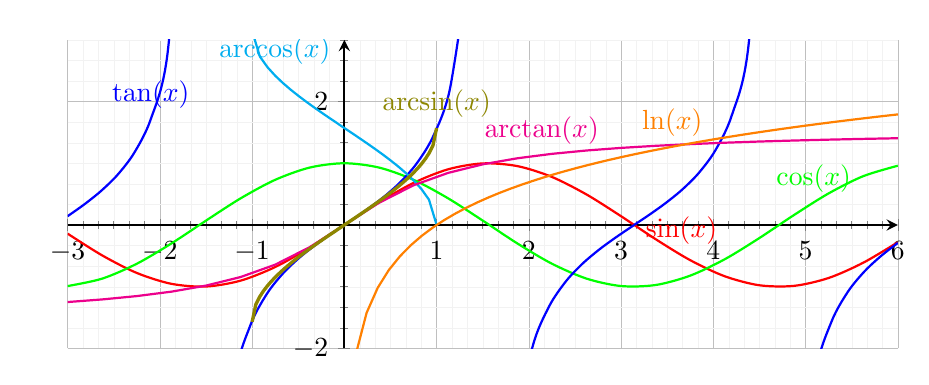
\begin{tikzpicture}
        \begin{axis}[
            axis lines = middle,
            domain = -3:6,
            ymin = -2,
            ymax = 3,
            width = \linewidth,
            height = 5.5cm,
            style = thick,
            grid = both,
            grid style = {line width=.1pt, draw=gray!10},
            major grid style = {line width=.2pt,draw=gray!50},
            minor tick num = 5,
            restrict y to domain=-10:10,
        ]
        
        \addplot[red, smooth]{sin(deg(x))} node[pos=0.75] (endofplotsquare1) {};
        \node [above,color=red] at (endofplotsquare1) {$\sin(x)$};

        \addplot[green, smooth]{cos(deg(x))} node[pos=0.9] (endofplotsquare2) {};
        \node [above,color=green] at (endofplotsquare2) {$\cos(x)$};

        \addplot[blue, smooth, samples=51]{tan(deg(x))} node[pos=0.05] (endofplotsquare3) {};
        \node [above,color=blue] at (endofplotsquare3) {$\tan(x)$};
        
        \addplot[cyan, domain=-1:1]{acos(x)/180*pi} node[pos=0.2] (endofplotsquare4) {};
        \node [above,color=cyan] at (endofplotsquare4) {$\arccos(x)$};

        \addplot[magenta] {atan(x)/180*pi} node[pos=0.6] (endofplotsquare5) {};
        \node [above,color=magenta] at (endofplotsquare5) {$\arctan(x)$};

        \addplot[olive, domain=-1:1, samples=51, style=very thick]{asin(x)/180*pi} node[pos=1] (endofplotsquare6) {};
        \node [above,color=olive] at (endofplotsquare6) {$\arcsin(x)$};

        \addplot[orange, domain=0.001:6, samples=51]{ln(x)} node[pos=0.8] (endofplotsquare7) {};
        \node [above,color=orange] at (endofplotsquare7) {$\ln(x)$};

        \end{axis}
    \end{tikzpicture}
\end{center}

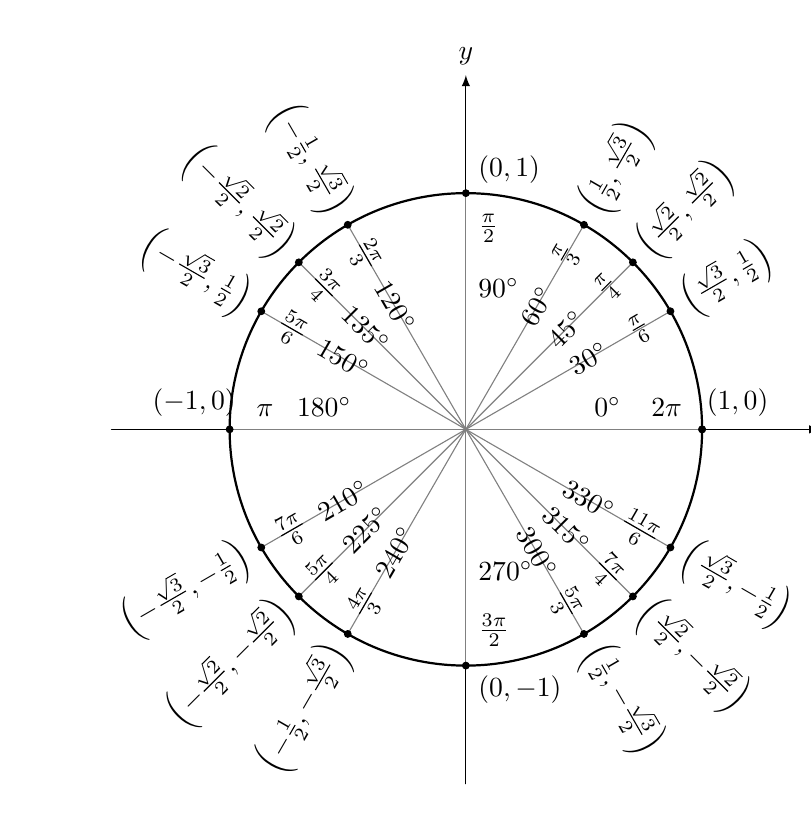
\begin{tikzpicture}[scale=3,cap=round,>=latex]
    \draw[->] (-1.5cm,0cm) -- (1.5cm,0cm) node[right,fill=white] {$x$}; % x axis
    \draw[->] (0cm,-1.5cm) -- (0cm,1.5cm) node[above,fill=white] {$y$}; % y axis
    
    % draw the unit circle
    \draw[thick] (0cm,0cm) circle(1cm);
    
    \foreach \x in {45,135, 225,315,0,30,...,360} { % <-- bissectrices added
      \draw[gray] (0cm,0cm) -- (\x:1cm); % lines from center to point
      \filldraw[black] (\x:1cm) circle(0.4pt); % dots at each point
    }
    
    % for the first and fourth quadrants
    \foreach \adeg/\radtext/\xc/\yc in {
      30/\frac{\pi}{6}/\frac{\sqrt{3}}{2}/\frac{1}{2},
      45/\frac{\pi}{4}/\frac{\sqrt{2}}{2}/\frac{\sqrt{2}}{2},
      60/\frac{\pi}{3}/\frac{1}{2}/\frac{\sqrt{3}}{2},
      300/\frac{5\pi}{3}/\frac{1}{2}/-\frac{\sqrt{3}}{2},
      315/\frac{7\pi}{4}/\frac{\sqrt{2}}{2}/-\frac{\sqrt{2}}{2},
      330/\frac{11\pi}{6}/\frac{\sqrt{3}}{2}/-\frac{1}{2}
    }
    {
      \draw (\adeg:0.6cm) node[rotate around={\adeg:(0,0)}] {$\adeg^\circ$}; % <-- rotate around key used
      \draw (\adeg:0.85cm) node[rotate around={\adeg:(0,0)}] {$\radtext$}; % <-- rotate around key used
      \draw (\adeg:1.025cm) node[rotate around={\adeg:(0,0)}, anchor=west] {$\left(\xc,\yc\right)$}; % <-- rotate around key used, radius changed, anchor key used
    }
  
    % for the second and third quadrants
    \foreach \adeg/\radtext/\xc/\yc in {
      120 / \frac{2\pi}{3} / -\frac{1}{2} / \frac{\sqrt{3}}{2},
      135 / \frac{3\pi}{4} / -\frac{\sqrt{2}}{2} / \frac{\sqrt{2}}{2},
      150 / \frac{5\pi}{6} / -\frac{\sqrt{3}}{2} / \frac{1}{2},
      210 / \frac{7\pi}{6} / -\frac{\sqrt{3}}{2} / -\frac{1}{2},
      225 / \frac{5\pi}{4} / -\frac{\sqrt{2}}{2} / -\frac{\sqrt{2}}{2},
      240 / \frac{4\pi}{3} / -\frac{1}{2} / -\frac{\sqrt{3}}{2}
    }
    {
      \draw (\adeg:0.6cm) node[rotate around={\adeg+180:(0,0)}] {$\adeg^\circ$}; % <-- rotate around key used
      \draw (\adeg:0.85cm) node[rotate around={\adeg+180:(0,0)}] {$\radtext$}; % <-- rotate around key used
      \draw (\adeg:1.025cm) node[rotate around={\adeg+180:(0,0)}, anchor=east] {$\left(\xc,\yc\right)$}; % <-- rotate around key used, radius changed, anchor key used
    }
    
    \foreach \adeg/\radtext/\xc/\yc in {0 / 2\pi / 1 / 0, 180 / \pi / -1 / 0}
    {
      \draw (\adeg:0.6cm) node[above=1pt] {$\adeg^\circ$};
      \draw (\adeg:0.85cm) node[above=1pt] {$\radtext$};
      \draw (\adeg:1.15cm) node[above=1pt] {$\left(\xc,\yc\right)$}; % <-- radius changed
    }
    
    \foreach \adeg/\radtext/\xc/\yc in {90 / \frac{\pi}{2} / 0 / 1, 270 / \frac{3\pi}{2} / 0 / -1}
    {
      \draw (\adeg:0.6cm) node[right=1pt] {$\adeg^\circ$};
      \draw (\adeg:0.85cm) node[right=1pt] {$\radtext$};
      \draw (\adeg:1.1cm) node[right=1pt] {$\left(\xc,\yc\right)$}; % <-- radius changed
    }
  \end{tikzpicture}

\subsection*{Derivatives and Integrals (\href{https://n.ethz.ch/~dcamenisch/summaries/}{src: dcamenisch})}
\renewcommand{\arraystretch}{1.5}
\begin{center}
\begin{tabular}{c|c}
    $\mathbf{F(x)}$ & $\mathbf{f(x)}$ \\
    \midrule
    $c$ & $0$ \\
    $x^a$ & $a \cdot x^{a - 1}$ \\
    $\frac{1}{a+1} x^{a + 1}$ & $x^a$ \\
    $\frac{1}{a \cdot (n + 1)} (ax + b)^{n + 1}$ & $(ax + b)^n$ \\
    $\frac{x^{a + 1}}{a + 1}$ & $x^a, \ a \neq -1$ \\
    $\frac{1}{x}$ & $-\frac{1}{x^2}$ \\
    $\sqrt{x}$ & $\frac{1}{2\sqrt{x}}$ \\
    $\sqrt[n]{x}$ & $\frac{1}{n}x^{\frac{1}{n} - 1}$ \\
    $\frac{2}{3}x^{\frac{3}{2}}$ & $\sqrt{x}$ \\
    $\frac{n}{n+1} x^{\frac{1}{n} + 1}$ & $\sqrt[n]{x}$ \\
    $e^x$ & $e^x$ \\
    $\ln(|x|)$ & $\frac{1}{x}$ \\
    $\log_a(|x|)$ & $\frac{1}{x \ln(a)} = \log_a(e^\frac{1}{x})$ \\
    $\sin(x)$ & $\cos(x)$ \\
    $\cos(x)$ & $-\sin(x)$ \\
    $\tan(x) = \frac{\sin(x)}{\cos(x)}$ & $\frac{1}{\cos^2(x)} = 1 + \tan^2(x)$ \\
    $\cot(x) = \frac{\cos(x)}{\sin(x)}$ & $\frac{1}{-\sin^2(x)}$ \\
    $\arcsin(x)$ & $\frac{1}{\sqrt{1 - x^2}}$ \\
    $\arccos(x)$ & $\frac{-1}{\sqrt{1 - x^2}}$ \\
    $\arctan(x)$ & $\frac{1}{1 + x^2}$ \\
    $\sinh(x) = \frac{e^x + e^{-x}}{2}$ & $\cosh(x)$ \\
    $\cosh(x) = \frac{e^x - e^{-x}}{2}$ & $\sinh(x)$ \\
    $\tanh(x) = \frac{\sinh(x)}{\cosh(x)}$ & $\frac{1}{\cosh^2(x)} = 1 - \tanh^2(x)$ \\
    $\frac{1}{f(x)}$ & $\frac{-f'(x)}{(f(x))^2}$ \\
    $a^{cx}$ & $a^{cx} \cdot c \ln(a)$ \\
    $x^x$ & $x^x \cdot (1 + \ln(x)), \ x > 0$ \\
    $(x^x)^x$ & $(x^x)^x (x + 2x \ln(x)), \ x > 0$ \\
    $x^{x^x}$ & $x^{x^x} (x^{x - 1} + \ln(x) \cdot x^x (1 + \ln(x)))$ \\
\end{tabular}

\begin{tabular}{c|c}
    $\mathbf{F(x)}$ & $\mathbf{f(x)}$ \\
    \midrule
    $\frac{1}{a} \ln(|ax + b|)$ & $\frac{1}{ax + b}$ \\
    $\frac{ax}{c} - \frac{ad - bc}{c^2} \ln(|cx + d|)$ & $\frac{ax + b}{cx + d}$ \\
    $\frac{1}{2a} \ln\left(\left| \frac{x-a}{x+a} \right|\right)$ & $\frac{1}{x^2 - a^2}$ \\
    $\frac{x}{2} \sqrt{a^2 + x^2} + \frac{a^2}{2} \ln(x + \sqrt{a^2 + x^2}) $ & $ \sqrt{a^2 + x^2} $ \\
    $\frac{x}{2} \sqrt{a^2 - x^2} - \frac{a^2}{2} \arcsin\left(\frac{x}{|a|}\right)$ & $\sqrt{a^2 - x^2}$ \\
    $\frac{x}{2} \sqrt{x^2 - a^2} - \frac{a^2}{2} \ln(x + \sqrt{x^2 - a^2}) $ & $\sqrt{x^2 - a^2}$ \\
    $\ln(x + \sqrt{x^2 \pm a^2})$ & $\frac{1}{\sqrt{x^2 \pm a^2}}$ \\
    $\arcsin\left(\frac{x}{|a|}\right)$ & $\frac{1}{\sqrt{a^2 - x^2}}$ \\
    $\frac{1}{a} \arctan\left(\frac{x}{a}\right)$ & $\frac{1}{x^2 + a^2}$ \\
    $-\frac{1}{a} \cos(ax + b)$ & $\sin(ax + b)$ \\
    $\cos(ax + b)$ & $-a\sin(ax + b)$ \\
    $\frac{1}{a} \sin(ax + b)$ & $\cos(ax + b)$ \\
    $\sin(ax + b)$ & $a\cos(ax + b)$ \\
    $-\ln(|\cos(x)|)$ & $\tan(x)$ \\
    $\ln (|\sin(x)|)$ & $\cot(x)$ \\
    $\ln\left(\left|\tan\left(\frac{x}{2}\right)\right|\right)$ & $\frac{1}{\sin(x)}$ \\
    $\ln\left(\left|\tan(\frac{x}{2} + \frac{\pi}{4})\right|\right)$ & $\frac{1}{\cos(x)}$ \\
    $\frac{1}{2} (x - \sin(x) \cos(x))$ & $\sin^2(x)$ \\
    $\frac{1}{2} (x + \sin(x) \cos(x))$ & $\cos^2(x)$ \\
    $\frac{1}{4}(\frac{1}{3}\cos(3x) - 3\cos(x))$ & $\sin^3(x)$ \\
    $\frac{1}{4}(\frac{1}{3}\sin(3x) + 3\sin(x))$ & $\cos^3(x)$ \\
    $\tan(x) - x$ & $\tan^2(x)$ \\
    $-\cot(x) - x$ & $\cot^2(x)$ \\
    $x \arcsin(x) + \sqrt{1 - x^2}$ & $\arcsin(x)$ \\
    $x \arccos(x) - \sqrt{1 - x^2}$ & $\arccos(x)$ \\
    $x \arctan(x) - \frac{1}{2} \ln (1 + x^2)$ & $\arctan(x)$ \\
    $\ln(\cosh(x))$ & $\tanh(x)$ \\
    $\ln(| f(x) |)$ & $\frac{f'(x)}{f(x)}$ \\
\end{tabular}

\begin{tabular}{c|c}
    $\mathbf{F(x)}$ & $\mathbf{f(x)}$ \\
    \midrule
    $x  (\ln(|x|) - 1)$ & $\ln(|x|)$ \\
    $\frac{1}{n+1} (\ln x)^{n+1} \quad \quad n \neq -1 $ & $ \frac{1}{x}(\ln x)^n$ \\
    $\frac{1}{2n} (\ln x^n)^{2} \quad \quad n \neq 0 $ & $ \frac{1}{x}\ln x^n$ \\
    $\ln(|\ln(x)|) \quad \quad x > 0, x \neq 1$ & $\frac{1}{x \ln(x)}$ \\
    $\frac{1}{b \ln(a)} a^{bx}$ & $a^{bx}$ \\
    $\frac{cx - 1}{c^2} \cdot e^{cx}$ & $x \cdot e^{cx}$ \\
    $\frac{1}{c}e^{cx}$ & $e^{cx}$ \\
    $\frac{x^{n + 1}}{n + 1} \left(\ln(x) - \frac{1}{n + 1}\right) \quad n \neq -1 $ & $x^n \ln(x)$ \\
    $\frac{e^{cx} \left(c \sin(ax + b) - a \cos(ax + b) \right)}{a^2 + c^2}$ & $\quad e^{cx} \sin (ax + b) $ \\
    $\frac{e^{cx} \left(c \cos (ax + b) + a \sin(ax + b) \right)}{a^2 + c^2}$ & $\quad e^{cx} \cos (ax+b)$ \\
    $\sin(x)\cos(x)$ & $\frac{\sin^2(x)}{2}$ \\
    $\frac{1}{2}(f(x))^2$ & $f'(x) f(x)$ \\
    $\sqrt{\pi}$ & $\int_{-\infty}^\infty e^{-x^2} \,dx$ \\
    $\frac{1}{a(n+1)}(ax+b)^{n+1}$ & $(ax+b)^n$ \\
    $\frac{(ax+b)^{n+2}}{(n+2)a^2} - \frac{b(ax+b)^{n+1}}{(n+1)a^2}$ & $x(ax)^n$ \\
    $\frac{(ax^p+b)^{n+1}}{ap(n+1)}$ & $(ax^p+b)^n x^{p-1}$ \\
    $\frac{1}{ap} \ln |ax^p + b|$ & $(ax^p + b)^{-1} x^{p-1}$ \\
    $\frac{ax}{c} - \frac{ad-bc}{c^2} \ln |cx +d|$ & $\frac{ax+b}{cx+d}$ \\
    $- x \cos (x)$ & $x \sin (x)$ \\
    $x \sin(x) + \cos (x)$ & $x \cos (x)$ \\
\end{tabular}
\end{center}

\end{document}
